\chapter{Supplementary material}
\label{ch:appendix}

% At most eight to ten pages: API contract excerpt, realm template excerpt, migration listing, raw evaluation tables.

\section{Regulatory clocks per regime}
\label{sec:appendix-clocks}

The deadlines section~\ref{sec:design-clocks} describes, as the engine's rules carry them.

\begin{figure}[H]
\centering
\small
\begin{tabular}{llrll}
\toprule
Regime & Clock & Count & Unit & Basis \\
\midrule
\code{EU\_PSD2\_CARD} & refund & 1 & business days & PSD2 art.~73(1) \\
 & resolution & 15 & business days & PSD2 art.~101(2) \\
\code{EU\_SEPA\_DIRECT\_DEBIT} & refund & 10 & business days & PSD2 art.~77(2) \\
 & resolution & 15 & business days & PSD2 art.~101(2) \\
\code{US\_REG\_E} & refund & 10 & business days & 12 CFR 1005.11(c)(2)(i) \\
 & resolution & 45 & calendar days & 12 CFR 1005.11(c)(2) \\
\code{US\_REG\_Z} & acknowledge & 30 & calendar days & 12 CFR 1026.13(c)(1) \\
 & resolution & 90 & calendar days & 12 CFR 1026.13(c)(2) \\
\bottomrule
\end{tabular}
\caption{The clocks each regime starts when a dispute opens (\code{domain/regime.go}). Extensions the law
permits for complex cases are not modelled; see section~\ref{sec:limitations}.}
\label{fig:clocks}
\end{figure}

\clearpage
\section{Ledger postings}
\label{sec:appendix-ledger}

The postings section~\ref{sec:design-ledger} describes, one row per state that causes one.

\begin{figure}[H]
\centering
\small
\begin{tabular}{L{5.5cm}L{4.1cm}L{2.4cm}L{1.6cm}}
\toprule
State entered & Posting & Debit & Credit \\
\midrule
any credit state & credit (disputed less liability) & suspense & customer \\
\code{PROVISIONAL\_CREDIT\_REVERSED} & reversal (outstanding) & customer & suspense \\
\code{CHARGEBACK\_WON} & recovery (outstanding) & recovery & suspense \\
\code{CHARGEBACK\_LOST}, no provisional credit & write-off (outstanding) & loss & suspense \\
\code{CLOSED}, outstanding & settlement, recovered or written off & recovery or loss & suspense \\
\bottomrule
\end{tabular}
\caption{Postings caused by entering a state (\code{domain/ledger.go}). ``Outstanding'' is the dispute's suspense
balance before the transition; a posting of zero is not written.}
\label{fig:ledger}
\end{figure}

\clearpage
\section{Operating the service}
\label{sec:appendix-operations}

Captured from the running system with \code{pnpm screenshot:ops} after a load run, so they can be retaken after a
change (section~\ref{sec:impl-observability}).

\begin{figure}[H]
\centering
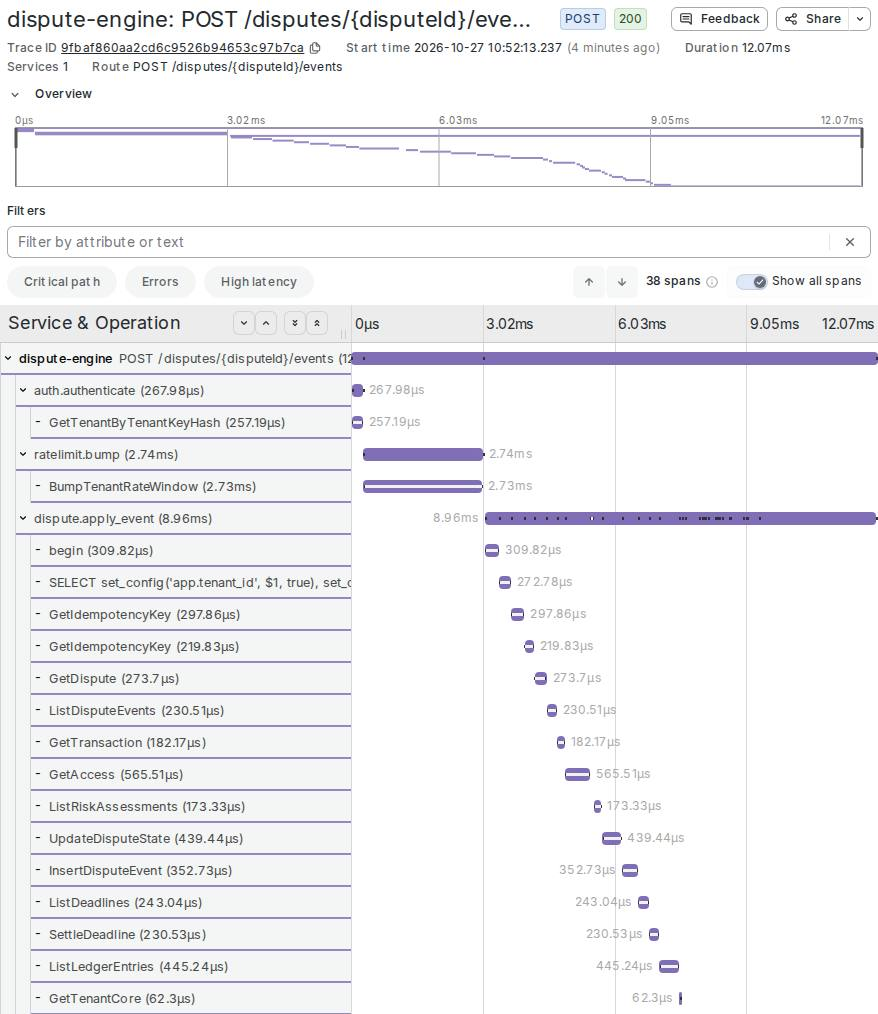
\includegraphics[width=0.85\textwidth]{trace.jpg}
\caption{One transition traced in Tempo: the request, authentication by tenant key, the rate-limit counter, the use
case, and each database statement it ran inside one transaction, 12~ms in total. The trace continues below the
crop with the ledger posting, the call to the simulated core and the commit.}
\label{fig:trace}
\end{figure}

\begin{figure}[H]
\centering
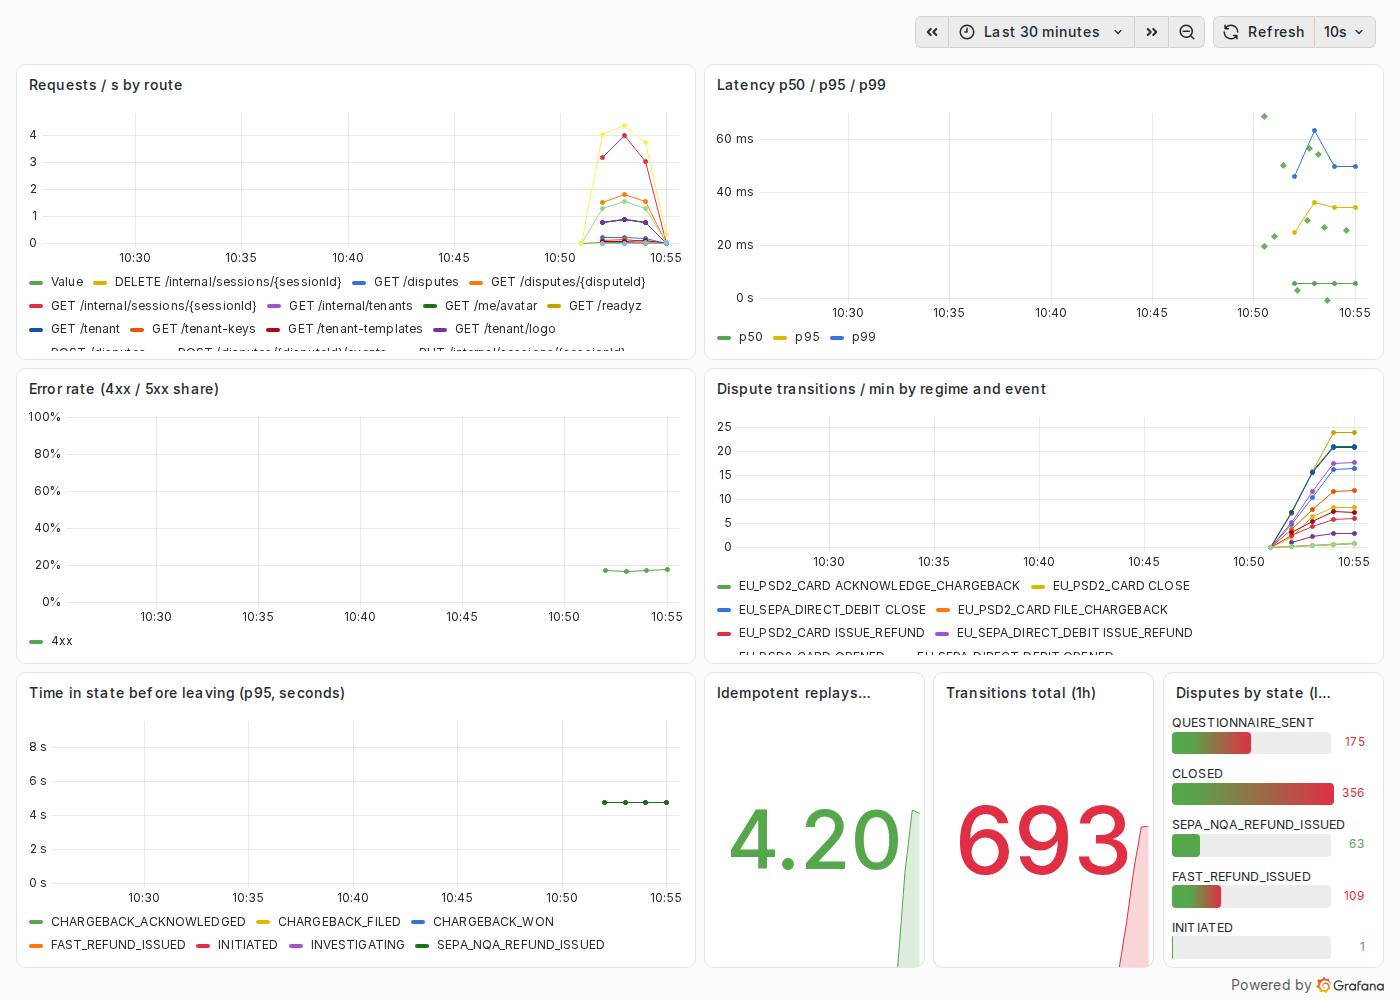
\includegraphics[width=\textwidth]{dashboard.jpg}
\caption{The engine's dashboard during a load run: request rate by route, latency percentiles, the share of client
and server errors (the 4xx line is the run's deliberate refused transitions), transitions by regime and event, time
spent in each state, and disputes by state.}
\label{fig:dashboard}
\end{figure}

\begin{figure}[H]
\centering
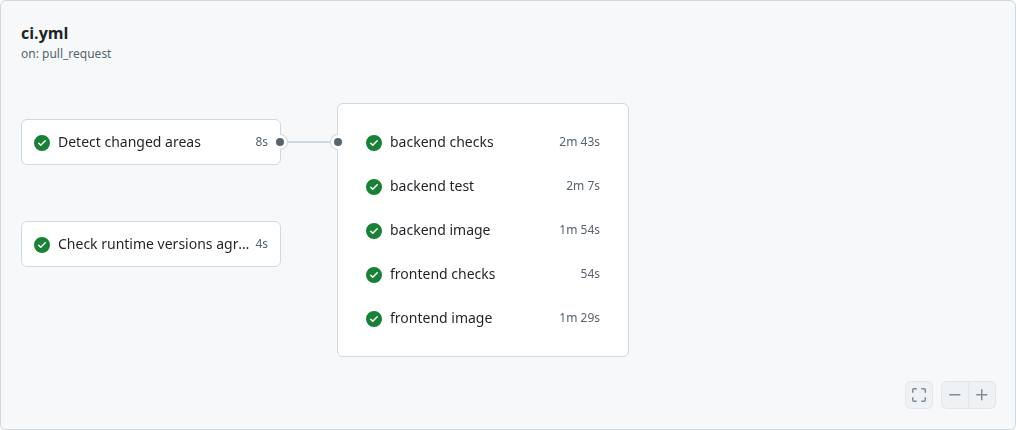
\includegraphics[width=0.8\textwidth]{ci.jpg}
\caption{The continuous-integration jobs of one pull request (the Go toolchain update of
section~\ref{sec:impl-ci}): change detection and the version check gate the backend and frontend jobs.}
\label{fig:ci}
\end{figure}
